\documentclass[10pt,conference]{IEEEtran}

\usepackage[pdftex]{graphicx}
\graphicspath{{res/}}
\usepackage{cite}
\usepackage{amsmath}
\usepackage{algorithm}
\usepackage{algpseudocode}
\usepackage{array}
\usepackage{tabularx}
\usepackage{amsfonts}

\usepackage{listings}
\usepackage{xcolor}
\lstdefinelanguage{json}{
    basicstyle=\normalfont\ttfamily\small,
    numbers=left,
    numberstyle=\scriptsize\color{gray},
    stepnumber=1,
    numbersep=8pt,
    showstringspaces=false,
    breaklines=true,
    frame=lines,
    backgroundcolor=\color{white},
    literate=
     *{0}{{{\color{blue}0}}}{1}
      {1}{{{\color{blue}1}}}{1}
      {2}{{{\color{blue}2}}}{1}
      {3}{{{\color{blue}3}}}{1}
      {4}{{{\color{blue}4}}}{1}
      {5}{{{\color{blue}5}}}{1}
      {6}{{{\color{blue}6}}}{1}
      {7}{{{\color{blue}7}}}{1}
      {8}{{{\color{blue}8}}}{1}
      {9}{{{\color{blue}9}}}{1}
      {:}{{{\color{black}{:}}}}{1}
      {,}{{{\color{black}{,}}}}{1}
      {\{}{{{\color{black}{\{}}}}{1}
      {\}}{{{\color{black}{\}}}}}{1}
      {[}{{{\color{black}{[}}}}{1}
      {]}{{{\color{black}{]}}}}{1},
}

\usepackage[caption=false,font=footnotesize]{subfig}
\usepackage{url}

\hyphenation{op-tical net-works semi-conduc-tor
             Sha-dow-socks Hys-te-ria Sing-box Xray-core
             sub-scrip-tion con-fig-u-ra-tion re-acha-bil-i-ty}

\tolerance=1500
\emergencystretch=12pt

\begin{document}

\title{PAVE: An Automated Pipeline for Reachability and Dynamic Analysis of Public Proxy Feeds}

\author{\IEEEauthorblockN{Reza Ahmadi}
\IEEEauthorblockA{\textit{Department of Computer Science} \\
\textit{University of Verona} \\
Verona, Italy \\
seyedmohammadreza.ahmadi@studenti.univr.it}}

\maketitle

\begin{abstract}
Modern internet users heavily rely on circumvention tools, yet free proxy configurations are frequently missing, unreachable, or affected by configuration staleness.
While tools exist to test proxy configurations from public subscription feeds, evaluating their absolute and comparative reachability at scale remains unaddressed.
This paper presents a large-scale empirical study investigating the viability, challenges, and architectural bottlenecks of automated free proxy configuration testing from public subscription feeds.
We design and implement the Proxy Analysis and Verification Engine (PAVE), a containerized, resource-conscious dynamic analysis infrastructure used to orchestrate, test, and segment proxy configurations across a massive subscription dataset.
Utilizing a multi-stage deduplication heuristic on public subscription repositories, we match and deduplicate proxy configurations collected from multiple Telegram channels and public aggregators.
Our empirical evaluation exposes 1,451 reachable configurations across five active proxy protocols, out of 115,042 deduplicated configuration records.
We benchmark five distinct proxy protocols (VLESS, VMess, Shadowsocks, Trojan, and Hysteria2) across 115,042 evaluation records.
The results quantify severe configuration availability scarcity and highlight systemic limitations in black-box proxy reachability, providing concrete insights into how hybrid static-dynamic analysis must evolve to mitigate configuration staleness.
\end{abstract}

\begin{IEEEkeywords}
Proxy Configuration, VPN Testing, Subscription Feed Analysis, Dynamic Analysis, Network Security.
\end{IEEEkeywords}

\section{Introduction}
In modern internet censorship circumvention, proxy protocols serve as the architectural foundation connecting restricted users to unrestricted remote services.
These configurations encapsulate distinct structural, communication, and authentication characteristics, such as server addresses, port numbers, encryption parameters, and proxy protocols (e.g., \texttt{VLESS}~\cite{xray_core}, \texttt{VMess}~\cite{v2ray}, \texttt{Shadowsocks}~\cite{shadowsocks}).
In this context, formal machine-readable subscription feeds establish an explicit contract between client-side applications and circumvention network infrastructure.

When discrepancies, omissions, or complete absences occur within these subscription feeds, the reliability of downstream circumvention activities, including automated black-box validation, reachability testing, and third-party integration, degrades sharply.
Despite the recognized utility of keeping configurations synchronized, a persistent misalignment remains between published and operational endpoints, frequently leading to a phenomenon known as configuration staleness~\cite{shadowsocks_gfw,gfw_encrypted}.

Researchers address missing or unreachable configurations using automated connectivity testing, which probes structural proxy definitions from runtime network behavior.
While various specialized client tools exist to test proxy configurations from subscription feeds, existing literature lacks systematic empirical data regarding how effectively these black-box testing mechanisms scale when subjected to realistic, unconstrained public subscription data.
Their absolute and comparative reachability remains unaddressed when deployed across a wide distribution of protocols.

This paper bridges this gap through a large-scale empirical study investigating the boundaries, viability, and operational challenges of automated black-box proxy configuration testing.
To execute this study under uniform testing constraints, we design and implement the Proxy Analysis and Verification Engine (PAVE).
PAVE serves as a containerized, resource-conscious dynamic analysis infrastructure used to orchestrate configuration fetching, test connectivity, and segment multi-protocol results across a massive target dataset.

\subsection{Research Objectives and Motivation}
Prior studies demonstrate that evaluating individual proxy protocols or small configuration samples in isolation fails to capture the systemic limitations, noise factors, and structural omissions found in production environments~\cite{khanvpn2018,perino2019,proxytorrent2018,proxies_unmasked}.
By exposing automated configuration testing pipelines to wide-reaching subscription datasets, this empirical study addresses three core motivations.
\begin{sloppypar}
\begin{LaTeXdescription}
    \item[Configuration Scarcity] Systematically identifying unreachable endpoints and structural mutations to illuminate the real-world severity of proxy and configuration staleness in the wild.
    \item[Benchmarking] Evaluating reachability rates, latency characteristics, and exit-node security profiles of distinct proxy protocols (VLESS~\cite{xray_core}, VMess~\cite{v2ray}, Shadowsocks~\cite{shadowsocks}, Trojan~\cite{trojan_gfw}, and Hysteria2~\cite{hysteria2_proto}) across identical, large-scale subscription records.
    \item[Bottlenecks] Quantifying how runtime constraints, security controls (e.g., SSL handshake failures), and connectivity parameterization affect automated black-box proxy testing workflows at scale.
\end{LaTeXdescription}
\end{sloppypar}

Given its global user base exceeding hundreds of millions and its extensive reliance on encrypted proxy communication~\cite{irblock2025,aryan2013iran}, the public subscription ecosystem serves as an ideal target domain for this empirical investigation.
Iran is one of the most heavily censored nations in the world~\cite{aryan2013iran}, with a large circumvention user base and a vast demand for free proxy subscription configurations~\cite{irblock2025,aryapour2025}.

\subsection{Problem Statement and Scope}
The execution of comprehensive, unguided proxy configuration testing at scale encounters several technical and architectural impediments.
First, testing tools detailed in the literature routinely operate under the assumption that valid proxy configurations are pre-existing and structurally accurate.
When these configurations are absent, connectivity mechanisms fail.
Second, manual configuration testing is inherently error-prone, labor-intensive, and non-scalable.

To conduct a scalable empirical study over thousands of configurations, disparate tools must be structured into a cohesive, orchestrated framework.
Furthermore, raw subscription data is inherently noisy, embedding duplicate configurations, expired endpoints, and credential-level duplicates that distort evaluation metrics if left unfiltered.
Finally, reproducible comparison requires building a reliable pipeline to map public subscription feeds to verifiable, testable proxy endpoints.

To address these challenges, we utilize a multi-stage deduplication heuristic on public subscription repositories to match and consolidate proxy configurations from Telegram channels and public aggregators.
Our empirical evaluation exposes 1,451 reachable configurations across five active protocols, out of 115,042 deduplicated evaluation records.
Ultimately, our results quantify severe configuration availability scarcity and highlight systemic limitations in black-box protocol reachability, providing concrete insights into how hybrid static-dynamic analysis must evolve to mitigate configuration staleness.

\subsection{Contributions}
Within this study, several critical aspects of proxy configuration testing and evaluation are introduced.
The main contributions are the following.

\begin{sloppypar}
\begin{LaTeXdescription}
    \item[Automated Experimental Pipeline] Design and development of a fully automated configuration testing pipeline capable of processing large datasets of proxy configurations without manual intervention.
    \item[Scalable Architecture] Implementation of a scalable system architecture that leverages configurable parallel container execution to reduce the overall testing time significantly.
    \item[Data Deduplication] Development of a multi-stage noise reduction mechanism that strictly filters duplicate and expired configurations, transforming raw subscription data into actionable information.
    \item[Repeatability] Engineering a deterministic system infrastructure that guarantees the repeatability of the experiments at every stage of the pipeline.
    \item[Standardized Data Enrichment] Introduction of a systematic approach to convert the tested results into standard formats (i.e., CSV/JSON) with geo-IP enrichment to match the exact structure of the analysis datasets.
    \item[Evaluation and Benchmarking] Establishment of a robust evaluation framework to compare the reachability results against the protocol specifications, alongside a comprehensive stability comparison of the related protocol clients and analysis tools.
    \item[Result Categories] Defining multiple configuration classes---unreachable, datacenter-hosted, and residentially-routed proxies---with security profiles covering DNS leak, IPv6 leak, and HTTP header leak detection.
\end{LaTeXdescription}
\end{sloppypar}

\section{Background and Related Work}
Before describing the pipeline, it is necessary to introduce preliminary notions concerning proxy protocol testing in the free subscription ecosystem.

\subsection{Dynamic Testing of Proxy Configurations}
Exploring any proxy configuration has many aspects and ways.
To understand how a proxy configuration works and how it communicates with its environment and network, there are two perspectives: static and dynamic.
The static approach investigates within the raw configuration string, and dynamic analysis runs a proxy client and observes its connectivity behavior.

All proxy configuration strings have a similar, well-defined structure for encoding parameters (the role of each field) and share the same encoding hierarchy.
Thanks to this standard, it is possible to examine the connection parameters of all configurations using a single approach, but there are some bottlenecks and limitations that make this approach impractical for most typical applications.
In the case of this study and the reachability analysis, many proxy servers are dynamically allocated and at runtime, and there is no final shape of the server state within the configuration string.

Due to limitations in configuration static analysis, dynamic analysis is more effective, but it requires an isolated system and a proxy client runtime environment.
The dynamic approach requires running the proxy client on the victim machine and allowing it to exhibit its connectivity behavior.
Due to the analysis of a large-scale dataset of proxy configurations, human interaction in dynamic analysis is totally impossible.
One of the most well-known languages for this purpose is Python~\cite{python_org}, a versatile scripting language used to orchestrate the automated testing pipeline in this project.

\subsection{Proxy Protocol Communication Architecture}
In this generation of the internet, for the secure exchange of users' data, everything is encrypted using protocols such as HTTPS and TLS~\cite{rfc8446}.
HTTPS enables encrypted communication over HTTP~\cite{rfc9110} via a secure TLS connection, and TLS operates in the background, conducting a handshake to establish secure encryption.
Without TLS, HTTP is unencrypted, allowing security analysts to view or steal information.

Security researchers use proxy protocols to circumvent censorship mechanisms~\cite{tor2004}.
They route their traffic through intermediary servers to access restricted data exchanged between the client and unrestricted destinations.
Censorship authorities in heavily filtered countries, such as Iran, deploy deep packet inspection and DNS~\cite{rfc1034} poisoning to intercept this communication~\cite{aryan2013iran}.
They apply protocol whitelisting and SNI-based filtering~\cite{rfc6066} to restrict the data exchanged between the user and unrestricted destinations~\cite{irblock2025,aryapour2025}.
The PAVE toolset provides a comprehensive suite of features for implementing this proxy testing architecture.
It dynamically launches and terminates proxy client processes on the fly, enabling the testing system to measure connectivity seamlessly.
Consequently, any data transferred over this tested connection becomes fully observable and measurable in terms of latency and exit-node identity.

\begin{figure}[htbp]
    \centering
    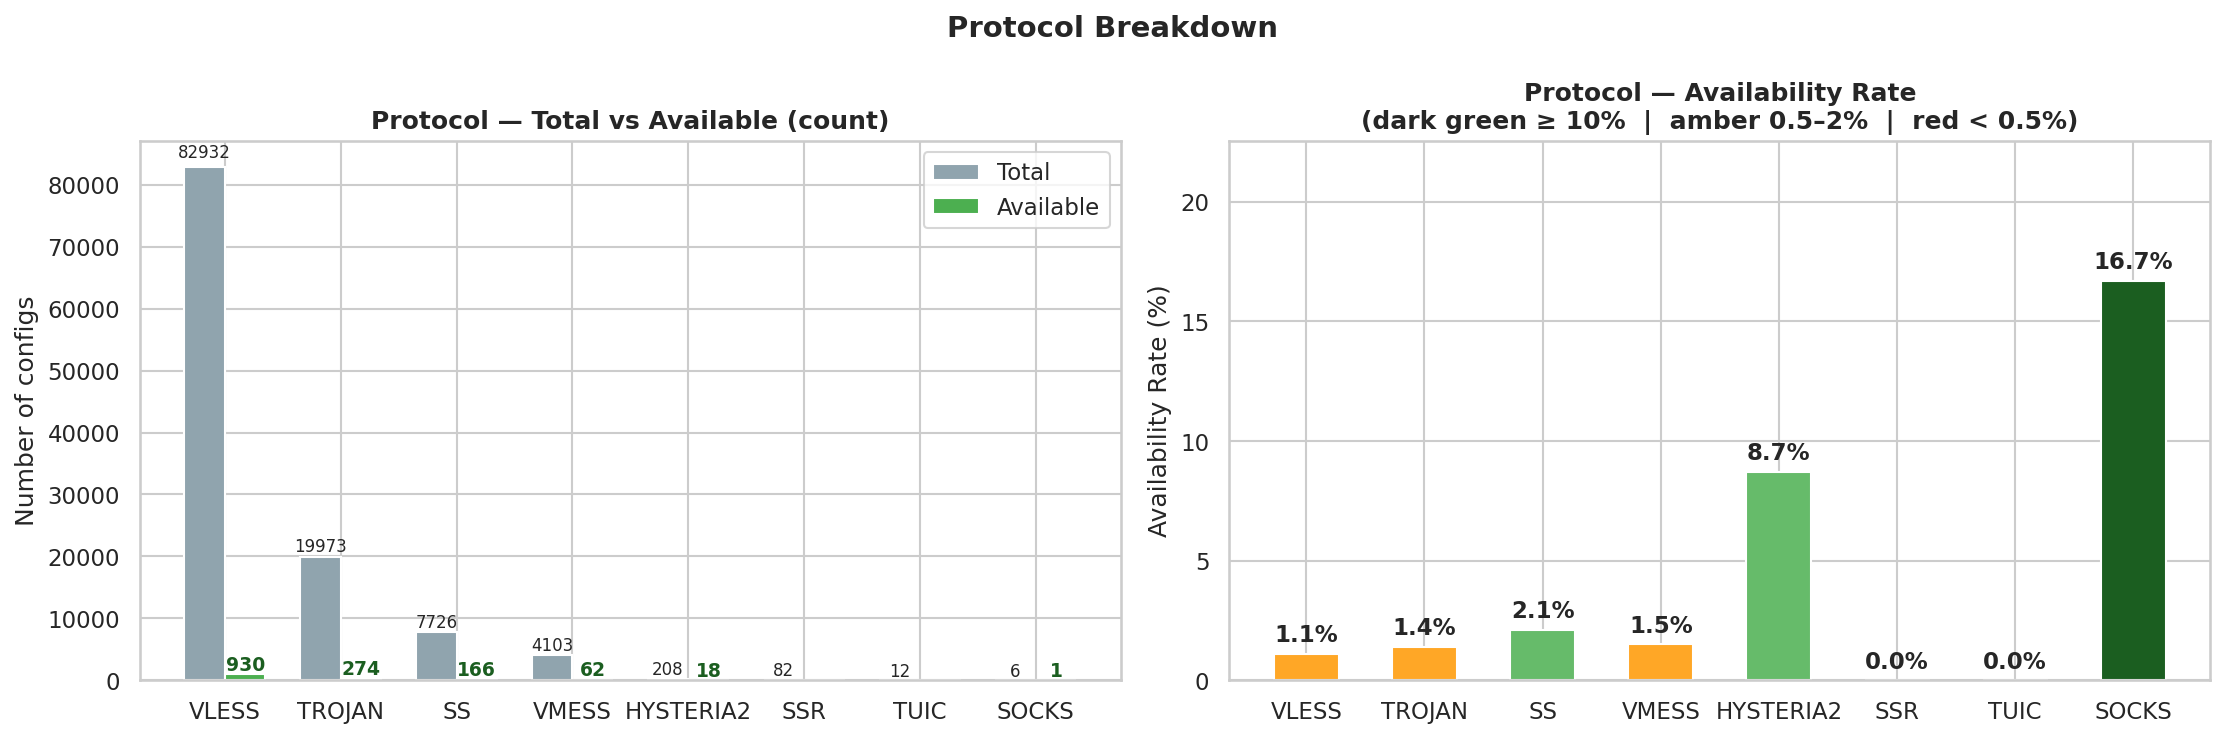
\includegraphics[width=0.9\columnwidth]{overview_availability.png}
    \caption{PAVE pipeline output overview: overall configuration availability (left) and exit-node type distribution among working configurations (right), across 115,042 tested records.}
    \label{fig:cps_overview}
\end{figure}

\subsection{Configuration Format Standards}
The most important part of a data comparison is the data structure.
There is a format used by proxy subscription services, called the URI configuration format, which is a Base64-encoded or plain-text representation of a proxy's connection parameters and authentication details.
Each configuration string contains all parameters between the client and the server; that is, all the proxy details include the server address, port, protocol, authentication credentials, transport layer, and encryption settings.

\begin{lstlisting}[language=json, numbers=none, caption={Generalized JSON schema representing the aggregated configuration dataset generated during the Subscription Profiling phase.}, label={lst:config_peeking_schema}]
{
  "channels": [
    {
      "source":
        "<String: Subscription Feed URL>",
      "configs": [
        "<String: Raw Proxy Config URI>",
        "..."
      ]
    },
    {
      "source": "...",
      "configs": [
        "..."
      ]
    }
  ]
}
\end{lstlisting}

At the end, the purpose is to convert raw subscription data to a human-readable format like CSV or JSON, a standardized, structured format.
With clean, structured information, it is possible to use a black-box approach to discover (or probe) the exact reachability of a configuration; then, as a Testing Process, it is possible to convert raw subscription data into critical knowledge for reuse.

\subsection{Existing Tools and Research Gaps}
The proxy configuration test requires several tools to work.
There are no tools available to run an end-to-end, fully automated test of this approach across all protocols, but some tools can technically help with part of it.

Xray~\cite{xray_core} is one of the most capable proxy cores for testing VLESS, VMess, Shadowsocks~\cite{shadowsocks_gfw}, and Trojan~\cite{trojan_gfw,trojanprobe2024} configurations.
Hysteria2~\cite{hysteria2_proto} is a modern UDP-based protocol client dedicated to the Hysteria2 protocol, offering low-latency connectivity and built-in congestion control.
Sing-box~\cite{singbox} is a universal proxy platform that supports TUIC~\cite{tuic} and ShadowsocksR~\cite{shadowsocksr} configurations and is designed to be easily integrated into automated testing pipelines.

Despite the availability of sufficient approaches and tools to test proxy configurations, an automated testing pipeline is lacking, especially across multi-protocol environments.
All these clients require manual configuration for each test.
When dealing with large-scale datasets, it is almost impossible to handle them manually.
Furthermore, the raw subscription data is not directly suitable for reachability testing, and some post-processing is required to make it noise-free and aligned with the base proxy servers.

\section{System Architecture}
We present now our Proxy Analysis and Verification Engine (PAVE).
One of the most important steps in running a testing experiment is having an automated system to organize tools and ensure they work together to generate test results.
While testing proxy configurations is already possible, these methods are not feasible for large datasets.
Therefore, a fully automated system capable of performing this procedure without supervision is required.
Implementing this system requires defining an approach and lifecycle for each configuration test, so the system can observe every test phase, from configuration fetching and deduplication through to saving connectivity results.
Multiple tests can run in parallel across a fixed number of containers, each independently processing its assigned configuration slice.
Running multiple test experiments in parallel, using tracking and advanced logging, and allowing any experiment to be repeated with the exact same behavioral parameters are additional reasons why implementing this automated test system is vital.
In this section, we will explain the system's orchestration and how we organize our tools to work together in a pipeline.
This process automates the steps from receiving the input subscription dataset to generating CSV and JSON files containing connectivity and security data.

\subsection{Overview of the Automated Experimental Pipeline}
The fundamentals of automated architecture are iteration.
In general, we have several proxy configurations in our datasets, and we need to follow the same process for each configuration.
For this purpose, we have chosen to use containerization tools such as Docker.
Meanwhile, running tests on the container helps us avoid concerns about multiple versions of the proxy client tools running and makes it suitable for migrating to another host system, which is particularly helpful for preventing conflicts, unwanted behavior, and errors.

In this approach, a fixed number of containers $N$ are launched in parallel on the host machine.
The entire deduplicated configuration list is partitioned into $N$ equal slices, and each container is assigned one slice to process independently.
Within each container, multiple test workers run concurrently to test the assigned configurations, combining parallelism at both the container and worker levels.

\subsection{Environment Configuration}
As we discussed, all testing will be done within a Docker container, and we can repeat this lifecycle for every configuration slice in the input dataset.
But behind the scenes, we need an actor to manage running containers.
Thanks to the available SDKs for Docker~\cite{docker}, the actor can be implemented as a script, providing sufficient flexibility.
The script is responsible for running all containers, waiting for each to complete its assigned slice, and transporting the needed parameters to each container, such as the total number of shards, the shard index, the worker count, and the output directory.
Managing container engines, such as Docker, is another mission of the script.

The primary step in enabling automated container execution is creating a base Docker image.
In this image, we provision a Debian-based environment and install essential dependencies, such as the Xray core~\cite{xray_core}, Hysteria2 client~\cite{hysteria2_proto}, Sing-box~\cite{singbox}, and Python~\cite{python_org}.

\begin{algorithm}[t]
\caption{Actor Script Orchestration and Parallel Container Execution}
\label{alg:actor}
\begin{algorithmic}[1]
    \State \textbf{Initialize} logging and output directory structures
    \State \textbf{Build} experiment base image $I_{exp}$
    \State \textbf{Fetch} all subscription URLs and deduplicate $\rightarrow$ $M$ configs
    \State \textbf{Set} $N \leftarrow$ number of containers (fixed)
    \State $chunk \leftarrow \lceil M / N \rceil$
    \For{each $i \in \{0, \ldots, N-1\}$ \textbf{in parallel}}
        \State \textbf{Run} $C_i$ with \texttt{--shards}~$N$ and \texttt{--shard}~$i$
        \State \textbf{Mount} shared config file and $shard\_i$ output directory
        \State \textbf{Stream} $C_i$ logs to $shard\_i.log$
    \EndFor
    \State \textbf{Wait} for all $N$ containers to complete
    \State \textbf{Merge} per-shard results into unified CSV/JSON
\end{algorithmic}
\end{algorithm}

\subsection{Parallel Container Orchestration}
One of the most important parts of the experiment that makes it significantly faster is the parallel execution of all containers simultaneously.
The script (Algorithm~\ref{alg:actor}) launches a fixed number $N$ of containers in parallel, each receiving a disjoint slice of the deduplicated configuration list.
Given $M$ total configurations and $N$ containers, each container receives $\lceil M/N \rceil$ configurations (the last container may receive fewer).
Within each container, $W$ concurrent test workers process the assigned slice, so the total concurrency across the experiment is $N \times W$.
The number of containers $N$ and workers per container $W$ are both configurable parameters, allowing the operator to tune parallelism to the available host resources.

\subsection{Intra-Container Lifecycle}
Each container runs the same testing script (Algorithm~\ref{alg:container}), but processes only its own slice of the configuration list determined by the shard index and total shard count passed as arguments.
Within the container, the system verifies the shard parameters and computes the exact slice boundaries before beginning any tests.
In this experiment, the system is also implemented to support multiple proxy client binaries in situations where different protocols require different runtime environments.

\subsubsection{Proxy Client Setup and Configuration}
Start the appropriate proxy client process for each configuration under test.
Configure key parameters so the proxy client runs properly in the test and container environments; the most important is to set the local SOCKS5~\cite{rfc1928} port to match the \texttt{curl}~\cite{curl} test client port that is used to measure exit-node connectivity and latency.
Then start another process to verify the configuration is accepted by the client and that the local proxy port is open.

\subsubsection{Automated Connectivity Testing}
Dynamic connectivity interaction is driven by the \texttt{curl}~\cite{curl}-based test harness.
The test harness is parameterized by an input parameter specifying the connection timeout in seconds.
It is parameterized to record the exit IP address, measure round-trip latency, and keep testing non-stop for all configurations in the shard.
Furthermore, the embedded script in the container is configured to capture the proxy client's log output, which is helpful for post-mortem analysis.

\subsubsection{Security Checks and Result Generation}
A dedicated test session is responsible for running DNS leak checks, IPv6 leak detection~\cite{vpn_survey2023}, proxy detection queries, and HTTP header leak detection (probing for \texttt{X-Forwarded-For} exposure) through each live proxy port.
Another parameter is set to a directory containing the connectivity and security results in CSV and JSON format.

\begin{algorithm}[t]
\caption{Containerized Environment Lifecycle}
\label{alg:container}
\begin{algorithmic}[1]
    \State \textbf{Load} shard parameters (--shard $i$, --shards $N$) from CLI arguments
    \State \textbf{Parse} each raw config URI into a \textit{ProxyConfig}
    \State \textbf{Deduplicate} configs at credential level
    \State \textbf{Slice} configs: $start \leftarrow i \cdot \lceil M/N \rceil$,\ $end \leftarrow \min(start + \lceil M/N \rceil,\ M)$
    \For{each $Config$ in $configs[start:end]$}
        \State \textbf{Select} appropriate proxy client via \textit{create\_tester()}
        \State \textbf{Launch} proxy client subprocess on local SOCKS5 port
        \State \textbf{Execute} \texttt{curl} through local port to get $exit\_ip$ and $latency\_ms$
        \If{connected}
            \State \textbf{Run} DNS leak, IPv6 leak, and proxy detection checks
        \EndIf
        \State \textbf{Terminate} proxy subprocess
    \EndFor
    \State \textbf{Enrich} results via batch geo-IP lookup
    \State \textbf{Export} results as \textbf{CSV} and \textbf{JSON}
\end{algorithmic}
\end{algorithm}

\section{Data Processing and Pipeline}
Raw data from subscription feeds is not suitable for analysis.
These feeds contain much noise and unnecessary configurations that should be excluded before analysis and evaluation.
The pipeline fetches data in real time.
The subscription decoder does not allow configuration exclusion during fetching, so it collects all proxy strings exchanged by every source.
Filtering after fetching lets us repeat the process when filtering and converting data, which needs further investigation.
Often, we do not know what noise or unnecessary data exists in the subscription feed, making post-fetch filtering necessary.

\subsection{Misinformation and Noise}
Looking at raw subscription data, it is clear that there are different types of noise we should remove before data analysis.
Discovered noises are as follows:

\subsubsection{Exact String Duplicates}
Such configurations appear across multiple subscription feeds and remain present in every experiment and captured dataset.
Multiple channels distribute the same configuration, and even when some servers are not reachable, these duplicates persist throughout the captured data.

\subsubsection{Credential-Level Duplicates}
Some functionally identical configurations appear with different display names or minor encoding variations.
For example, two configuration strings for the same server at the same port with the same authentication credentials but different \texttt{name} fields must be considered the same entry.
To find this noise, look for configurations with matching \texttt{protocol|server|port|auth} tuples, for example:
\begin{itemize}
    \item \textbf{Transport-Layer Variants:}
    \begin{itemize}
        \item \textit{Encoding:} Base64-encoded vs.\ plain-text URI representation of the same credentials.
        \item \textit{Display name:} Different \texttt{\#name} suffixes appended to the same underlying endpoint.
    \end{itemize}
    \item \textbf{Configuration and Constants:}
    \begin{itemize}
        \item \textit{Remote Configurations:} Endpoints sharing the same server IP, port, and UUID but different transport or TLS options that do not affect the underlying server identity.
    \end{itemize}
\end{itemize}

\subsubsection{Analytics and Telemetry Channels}
Modern Telegram channels integrate third-party bots and aggregators to improve the quality of their distribution.
Consequently, captured subscription data often includes proxy strings from external sources that do not reflect a single operator's core infrastructure.
Because they are configuration strings related to other operators' endpoints, it is feasible to skip them and consider them as noise data.
Most of these configurations are related to advertising and re-broadcasting services.
Before any post-study analysis of the captured subscription data for each channel, a priori prediction of comprehensive exclusion lists is infeasible due to the dynamic nature of third-party subscription traffic.
After the fetch step, it is not clear what the exact shape of the list is.
For this reason, before scripting the filtering of the captured data, we need an additional step to investigate and identify the exact base URLs of services that are not vital to the analysis.
In the next section, the Subscription Profiling approach will be discussed to show how these noises are discovered and removed before analysis.

\subsection{Subscription Profiling}
Subscription Profiling is an approach to quickly view all captured configurations.
In the System Architecture section, it is clear that after completing the experiment on a subscription dataset, a list of raw configuration strings will be generated, each corresponding to a subscription source in the dataset.
In Subscription Profiling, two or more automated scripts will be applied with almost identical missions and approaches on captured subscription data.
At the first level, a script crawls all the subscription responses and creates a large dataset of all the configurations accessed from all candidate sources in the experiment.
It could be a JSON Array within a JSON Object, containing multiple array items; each item represents a configuration list for each subscription source.

After this step, a quick glance at the generated dataset reveals the number of subscription sources collected and the configurations they contain.
The first prepared dataset contains a large amount of noisy data, including the two types discussed in the previous part.
Furthermore, in this step, hidden and unrecognizable noisy configurations are also discoverable, adding to the exclusion list for the next process.
After the next process and filtering, the new file contains almost 100 percent pure information.
With respect to the captured data, it is possible to see some of the configurations removed within the second process and filter, which means all the captured configurations of that source were kind of noise, which is due to some situations, such as: the candidate subscription was not decodable due to some problems like a mismatched Base64 padding, in some cases the configuration contained an unsupported protocol or for security reasons the configuration URI could not be parsed into a valid structure.

\subsection{Noise Reduction Process On Subscription Data}
To ensure the integrity of subsequent analysis, captured subscription data must undergo rigorous noise reduction.
Leveraging the explicit exclusion lists generated during the Subscription Profiling stage, a dedicated automated script systematically parses the aggregated dataset.
For every candidate configuration, the script identifies and excises non-functional entries and irrelevant credential duplicates.
Crucially, to preserve experimental repeatability, this process does not mutate the original subscription data.
Instead, it generates a distinct, noise-free configuration list, ensuring the raw captured data remains immutable and accessible for future auditing and review.

\subsection{Configuration Segmentation by Protocol}
The study captured subscription feeds that demonstrate that each source may contain multiple proxy protocols, even after removing noise.
In fact, it shows that the configuration sets for those sources are split across several distinct protocols, such as \texttt{vless://}, \texttt{vmess://}, and \texttt{trojan://}, all of which are present in the captured subscription data, and the philosophy of configuration segmentation by protocol is defined accordingly.
Also, discovering the protocol distribution would be impactful for two other reasons in the evaluation system.
The first is that for many proxy client tools, from raw URI to live connection, the protocol type is required; the second is that before the testing step, when matching two configuration records, a smaller protocol-homogeneous dataset makes the matching process faster and lighter.
An automated script can lead this process.
The script would crawl all the configuration strings iteratively.
Within each iteration, it identifies all distinct protocols and creates a filtered list for each.
For better management of the configuration records and easier identification of their relatives, the created lists would use the same name as the original source feed, with a protocol suffix for separation; for instance, \texttt{source.txt} with two protocols would be \texttt{source\_vless.txt} and \texttt{source\_trojan.txt}.

\subsection{Geo-IP Enrichment from Connectivity Results}
Every tested configuration produces a live exit-node IP address upon successful connection.
In fact, a connectivity result record is a CSV-formatted archive that the testing system uses to record all network activity during the proxy handshake or curl request.
It acts as a detailed, chronological log of the conversation between the PAVE client and a remote exit server.
The connectivity result contains all the details of the exchange, including exit IP address, latency in milliseconds, DNS~\cite{rfc1034} resolver IP, IPv6~\cite{rfc8200} exit address, and proxy detection flags.
The most important data for creating a geo-enriched analysis record is the exit IP, allowing each configuration to be attributed to a country, city, ASN, and datacenter classification.
Enriching connectivity results with geo-IP metadata is mandatory for us because the enriched record serves as a standard benchmark for formal proxy analysis, geographic distribution study, and security evaluation.

\section{Experimental Settings}
In this section, the tools used for testing and analysing proxy configurations are discussed.
The main objective is to define the tools and compare them, and then to define the scoring and metrics system for evaluating the PAVE system.

\subsection{Protocol Testing Tools}
Protocol testing tools are designed to automatically connect to a proxy server using a specific protocol and measure reachability and latency.
These tools use various subprocess managers and local SOCKS5 port bindings to interact with proxy servers and produce a structured result describing the connection outcome, exit IP, and measured latency.

\subsubsection{Xray-Based Tester}
Xray~\cite{xray_core} is a tool developed in Go~\cite{golang}.
Although this tool is based on Go, it supports a robust command-line interface (CLI) integration and is highly practical for use with PAVE, which is developed in Python.
This tool supports automated path parameterization for VLESS and VMess protocols, which is one of the most critical features for configuration testing.
It allows the tool to dynamically parse configuration URIs to detect transport parameters (like WebSocket~\cite{rfc6455} or gRPC~\cite{grpc} paths and UUIDs) and instantiate them into a running proxy process.
For instance, a URI with \texttt{type=ws\&path=/api} parameters is converted into a running Xray process with the correct WebSocket transport configuration.
This prevents the generation of thousands of failed connection attempts in the final evaluation.
This tool also supports TLS certificate pinning bypass, built-in timeout controls, and native noise reduction by rejecting malformed configurations before attempting a connection.

\subsubsection{Hysteria2-Based Tester}
Hysteria2~\cite{hysteria2_proto} is the most compatible tool with the Hysteria2 protocol in theory, and it is developed and designed to do specialized connection establishment from Hysteria2 configuration URIs to live SOCKS5~\cite{rfc1928} proxy tunnels.
This Go-based tool has a straightforward CLI and is designed to be easily integrated into the PAVE pipeline.
All connections will be established using the QUIC~\cite{rfc9000}-based Hysteria2 transport, the most recent high-performance proxy transport.
It supports sensitive data handling, which means that by using the \texttt{-c} (config file) command-line flag, it will parse the actual captured authentication tokens.
Like the other protocol runners, this tool requires the orchestrator to poll the local SOCKS5 port for readiness before accepting connections, as no callback or event notification system is provided.

\subsubsection{Sing-box-Based Tester}
Sing-box~\cite{singbox} is a universal proxy platform developed as a community-maintained project.
This tool is designed for automated black-box connectivity testing of multiple proxy protocols.
It interacts with the proxy server solely through standard protocol handshakes, without requiring access to the server's source code.
The only requirement is a valid proxy configuration URI of the protocol being tested.
The platform offers multiple components and features to assist researchers, practitioners, and developers in implementing custom testing strategies.
PAVE generates a sing-box JSON configuration from the parsed proxy URI, launches sing-box as a subprocess on a local SOCKS5 port, polls for readiness, and measures connectivity via \texttt{curl}.

\subsection{Analysis and Evaluation Frameworks}
Several analysis frameworks used in this project are discussed in this section, along with their features and capabilities.
These tools are designed to compare two configuration evaluation records and identify differences in reachability rates, latency distributions, geographic concentrations, and security profiles.
The main tools discussed are Pandas~\cite{pandas}, Scikit-learn~\cite{scikit_learn}, and PyTorch~\cite{pytorch}.
These tools are integrated outside the PAVE pipeline, as they are used for post-processing and analysis of the generated connectivity records.

\begin{table}[t]
\centering
\caption{Comparative analysis of features across proxy protocol testing tools.}
\label{tab:proto_tester_comparison}
\renewcommand{\arraystretch}{1.4}
\resizebox{\linewidth}{!}{%
\begin{tabular}{|l|c|c|c|}
\hline
\textbf{Feature} & \textbf{Xray} & \textbf{Hysteria2} & \textbf{Sing-box} \\ \hline
\textbf{Language} & Go & Go & Go \\ \hline
\textbf{Protocols} & VLESS/VMess/SS/Trojan~\cite{xray_core,v2ray,shadowsocks,trojan_gfw} & Hysteria2~\cite{hysteria2_proto} & TUIC/SSR~\cite{tuic,shadowsocksr} \\ \hline
\textbf{CLI} & High (poll-ready) & Med (poll-ready) & High (JSON-cfg) \\ \hline
\textbf{Auto-Param.} & UUID / WS-path & URI-based & JSON-based \\ \hline
\textbf{Noise Reduction} & Built-in & Start failure & Config validation \\ \hline
\textbf{TLS Support} & Yes (Reality/TLS) & Yes (QUIC) & Yes (TLS) \\ \hline
\textbf{Target Use Case} & General & High-speed & Universal \\ \hline
\end{tabular}%
}
\end{table}

\subsection{Threats to Validity}
In this section, potential threats to the validity of the experimental results are discussed, categorized into external, internal, and construct validity.

The primary threat to external validity is the selection of target subscription feeds.
While the experiment includes a variety of proxy protocols, the results may not generalize to all proxy architectures, such as WireGuard or OpenVPN.
Furthermore, the reliance on captured connectivity results means that the quality of the reachability analysis is directly bounded by the coverage of the initial subscription collection.

Internal validity may be affected by the temporal nature of proxy configuration availability.
Although these configurations were tested at a specific point in time, infrastructure changes in the proxy server environment could lead to false positives or negatives during the evaluation phase.
Additionally, the timeout parameters for the connectivity tests were kept at default values, which may not be optimal for every target server.

Construct validity concerns whether the comparison metrics accurately reflect the system's performance.
The use of automated geo-IP enrichment tools like ip-api.com~\cite{ipapi} provides a standardized measure of exit-node characteristics, but these tools may differ in their classification of datacenter versus residential networks, potentially affecting the final evaluation scores.

\section{Dataset and Ground Truth}
In this section, how to prepare required datasets to run and evaluate PAVE is discussed.
Fundamentally, PAVE requires a dataset of proxy configurations and after ending the pipeline of the test, it is required to compare generated results with the expected ground truth.

\subsection{Ground Truth Definition}
Evaluation of the PAVE outputs demands preparing specific information to compare.
Basically, for evaluation of the system, the shape of output records such as exit IP, latency, and protocol should be controlled.
Every difference is meaningful within this comparison.
Generally, comparison of two configuration records will find three types of configurations:
\begin{itemize}
    \item \textbf{Unreachable:} Configurations that PAVE could not connect through.
    \item \textbf{Datacenter:} Configurations whose exit IP belongs to a known datacenter or hosting range.
    \item \textbf{Residential:} Common configurations present in tested records with residential exit nodes.
\end{itemize}

\subsection{Public Subscription Repositories}
It is expected to run PAVE first, then investigate for corresponding reachability results, but after many efforts in this project, the experiment demonstrates that random selection of candidate subscription feeds does not guarantee availability of reachable proxy endpoints.
For this reason, before running the PAVE, it is necessary to investigate target candidate subscription sources.
There are many official and unofficial sources that could be sources of proxy configuration ground truth~\cite{perino2019,proxytorrent2018}.
Some public Telegram channels publish their official proxy configurations corresponding to their services, and there are also open-source communities that try to collect proxy configurations from official sources or manual capturing.

The most comprehensive unofficial source is Telegram-based subscription aggregators.
These services contain official and unofficial proxy configurations that are available to the public.
These aggregators offer practical features for investigating configurations, and the raw configuration feeds are available on their public Telegram channels, which are used in this project.
The \texttt{barry-far/V2ray-config}~\cite{barry_far_v2ray} repository is a comprehensive collection of proxy configurations from various public subscription channels, including protocol-separated feeds and combined subscription lists maintained by a community contributor.
This project uses it as the primary source for proxy configuration URIs across VLESS, VMess, Trojan, Shadowsocks, and ShadowsocksR~\cite{shadowsocksr} protocols.
The \texttt{ebrasha/free-v2ray-public-list}~\cite{ebrasha_v2ray} repository provides a broad set of free proxy configurations collected from multiple sources and maintained by EbraSha.
This project uses it as a supplementary source for additional multi-protocol proxy configuration URIs corresponding to the candidate subscription feeds.

The most critical part of configuration selection is related to choosing reachable and up-to-date proxy endpoints.
Fundamentally, within open-source subscription repositories, there is no possibility to filter only configurations that are currently reachable.
For this reason, an automated script is designed to check each configuration and try to find out if it is reachable or not.
The script checks each configuration for specific connectivity attributes, multiplies every positive signal with its respective predefined weight, and then calculates a score for each configuration.
If the score is higher than a specific threshold, the configuration is considered as reachable and added to the list of working proxy endpoints for the experiment.

\subsection{Configuration Dataset Selection}
The selection of proxy configurations for the experiment is a critical step.
For each subscription feed, it is required to find the corresponding proxy server that uses the protocol described in that configuration URI.
Because of the large number of available configuration URIs, it is not possible to find the corresponding server for each configuration by manual testing; for this reason, an automated script is designed to test each configuration programmatically.
Each configuration URI is parsed by protocol type, and if the protocol is supported by one of the available proxy client tools, it is used as an input to the connectivity test.
At the end of this process, a dataset of test results is prepared, where each configuration URI corresponds to zero, one, or more successful connectivity records.

\section{Results and Discussion}
This section presents the results obtained from executing the PAVE pipeline.
The evaluation focuses on the reachability of the configurations, the protocol distribution of the results, and the performance metrics of the system.
The results are analyzed using various comparative tools, specifically Pandas~\cite{pandas}, Scikit-learn~\cite{scikit_learn}, Matplotlib~\cite{matplotlib}, and PyTorch~\cite{pytorch}, to provide a comprehensive and multi-faceted assessment.

\subsection{Discovered Reachable Configurations}
The result of running the connectivity testing system on the collected subscription dataset produced \textbf{115,042} unique deduplicated configuration records, of which \textbf{1,451} were reachable at the end.
After the downloaded configuration list occupied about \textbf{5 MB} on the host machine storage, a \textbf{15-second} connection timeout was applied per configuration, and \textbf{1,451} were confirmed reachable at the end.
We ran our experiment with \textbf{20} parallel containers, each processing an equal slice of the configuration dataset with \textbf{50} concurrent workers.

\begin{figure}[htbp]
    \centering
    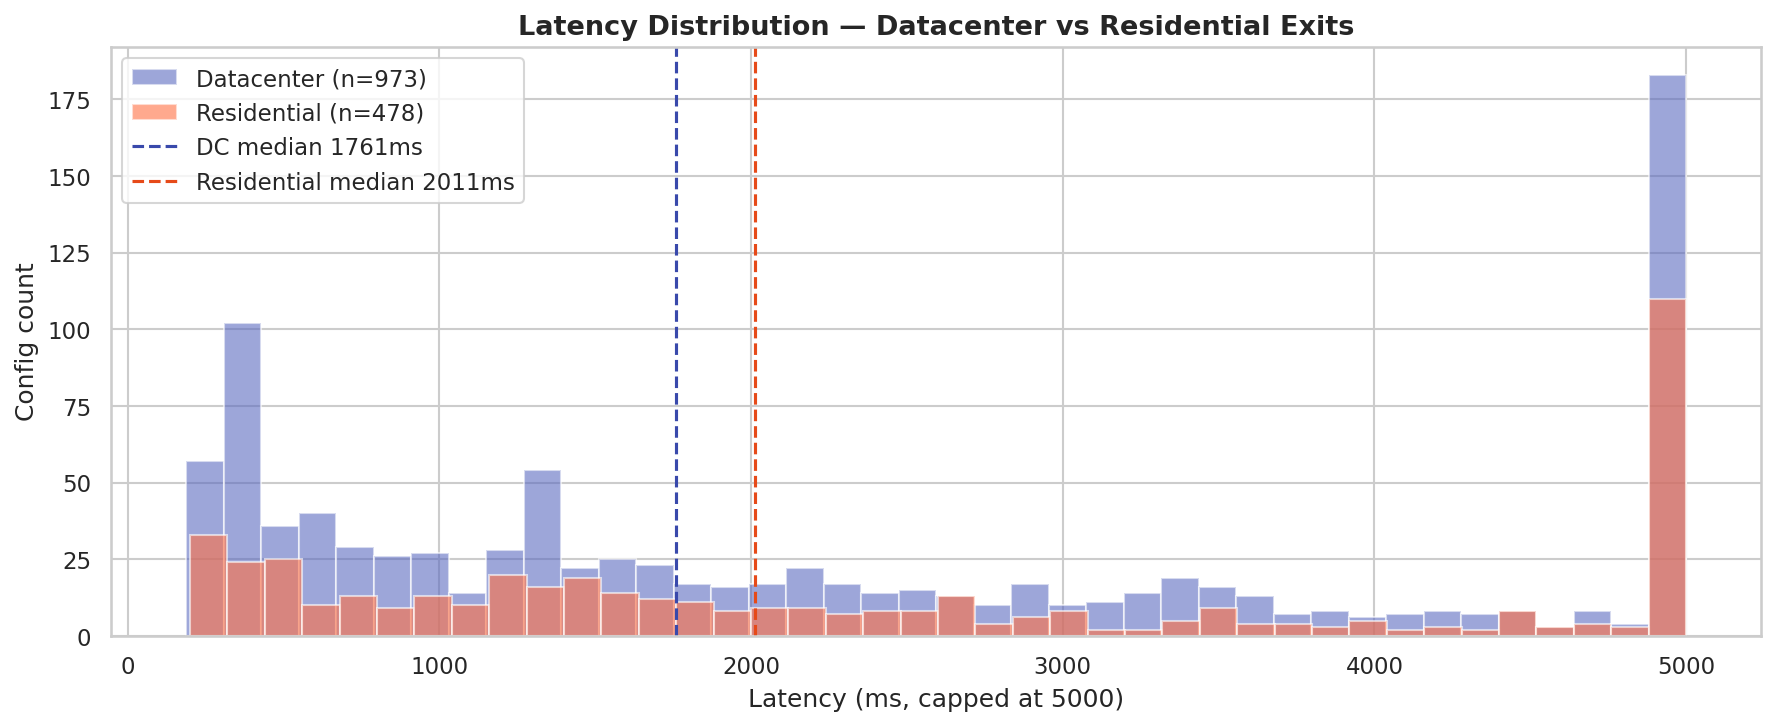
\includegraphics[width=0.9\columnwidth]{protocol_breakdown.png}
    \caption{Protocol breakdown: total configuration count vs.\ reachable count per protocol (left) and availability rate per protocol (right). Hysteria2 achieves the highest meaningful availability rate at 8.65\%.}
    \label{fig:protocol_breakdown}
\end{figure}

\begin{table}[t]
\centering
\caption{Total reachable configurations per proxy protocol.}
\label{tab:matched_proto_summary}
\renewcommand{\arraystretch}{1.3}
\begin{tabular}{l c c c}
\hline
\textbf{Protocol} & \textbf{Total} & \textbf{Reachable} & \textbf{Rate} \\
\hline
\textbf{VLESS}      & 82,932 & 930  & 1.12\% \\
\textbf{Trojan}     & 19,973 & 274  & 1.37\% \\
\textbf{SS}         & 7,726  & 166  & 2.15\% \\
\textbf{VMess}      & 4,103  & 62   & 1.51\% \\
\textbf{Hysteria2}  & 208    & 18   & 8.65\% \\
\textbf{SSR}        & 82     & 0    & 0.00\% \\
\textbf{TUIC}       & 12     & 0    & 0.00\% \\
\textbf{SOCKS}      & 6      & 1    & 16.67\% \\
\hline
\textbf{Total}      & 115,042 & 1,451 & 1.26\% \\
\hline
\end{tabular}
\end{table}

The above table shows the reachability rate, crash-free operation, and compatibility of protocol testing tools for connecting through each proxy configuration.

\subsection{Configuration Coverage Analysis}
By analyzing in detail the results of connectivity records, there are several vital information points.
Generally \textbf{115,042} records about the entire connectivity testing process are recorded by the PAVE pipeline.

\begin{table}[t]
\centering
\caption{Distribution of failure reasons across non-reachable configurations.}
\label{tab:failure_reason_distribution}
\renewcommand{\arraystretch}{1.2}
\begin{tabular}{l r}
\hline
\textbf{Failure Reason} & \textbf{Total Records} \\
\hline
Host unreachable             & 44,384 \\
SSL handshake failed         & 29,220 \\
Timeout                      & 20,516 \\
xray failed to start         & 19,319 \\
sing-box failed to start     &     74 \\
hysteria2 failed to start    &     60 \\
curl error 60                &      7 \\
curl error 97                &      5 \\
SOCKS proxy error            &      4 \\
curl error 18                &      2 \\
\hline
\textbf{Total}               & \textbf{113,591} \\
\hline
\end{tabular}
\end{table}

These results show that the majority of the failure records are generated by host-level unreachability and connection timeouts, while SSL handshake failures constitute a significant third category.
The cause of the gap between the number of records generated by host-unreachable and timeout compared to the other failure types is that most published proxy configurations are no longer actively maintained and their servers have gone offline.
The sparsity of reachable records generated by different protocol testing tools is different.

\begin{table}[t]
\centering
\caption{Exit node profile of reachable configurations.}
\label{tab:exit_node_profile}
\renewcommand{\arraystretch}{1.2}
\begin{tabular}{|l|c|c|c|}
\hline
\textbf{Category} & \textbf{Count} & \textbf{Pct.} & \textbf{Med.\ Latency} \\ \hline
Datacenter exit   & 973 & 67.1\% & -- \\ \hline
Residential exit  & 478 & 32.9\% & -- \\ \hline
Blacklisted IP    & 808 & 55.7\% & -- \\ \hline
Proxy-detected    & 814 & 56.1\% & -- \\ \hline
\end{tabular}
\end{table}

\subsection{Protocol Comparative Analysis}
These results demonstrate that Hysteria2 is the most robust protocol to provide reachable proxy configurations.
It has found 18 reachable endpoints in a dataset of 208 configurations, yielding an 8.65\% availability rate.
SS follows with 166 reachable from 7,726 at 2.15\%, and VMess with 62 reachable from 4,103 at 1.51\%.
At the end, VLESS has the most entries in the dataset but also the most fragile reachability in comparison to the other protocols at 1.12\%.

In the geographic distribution of reachable configurations, the results are significantly different.
Germany is the most represented exit country with 274 working configurations, with a large gap with respect to other countries.
The Netherlands follows with 190 reachable configurations, and the United States with 181.
France and Singapore follow with 138 and 79 respectively.

\begin{figure}[htbp]
    \centering
    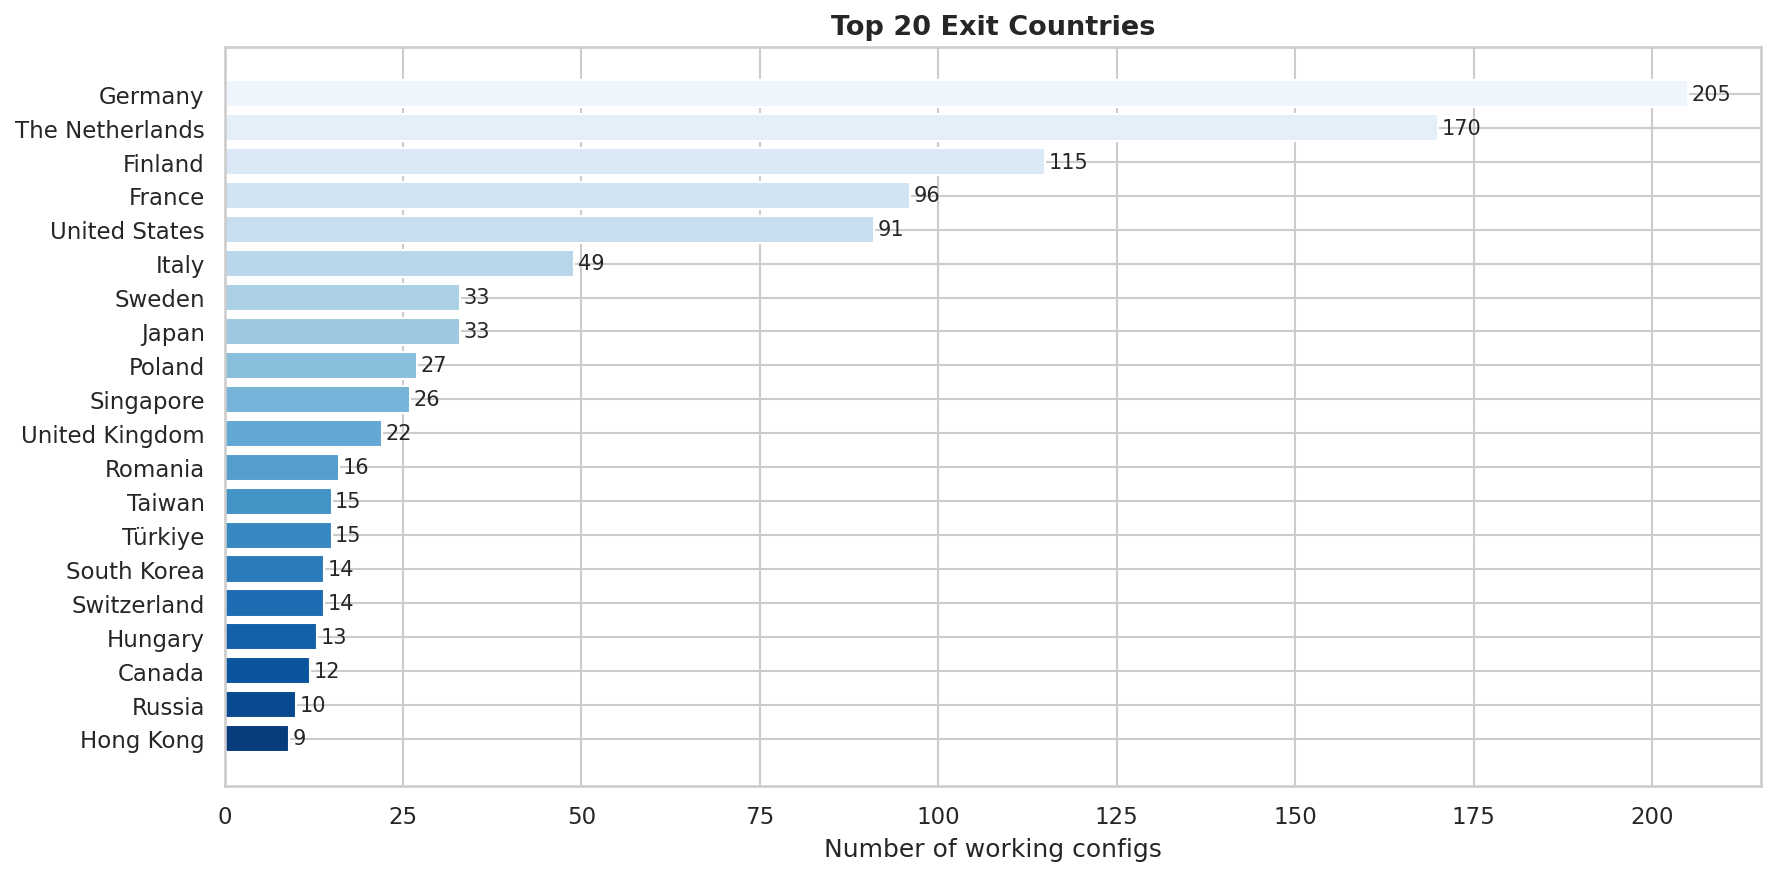
\includegraphics[width=0.9\columnwidth]{geo_distribution.png}
    \caption{Top 20 exit countries for reachable configurations. Germany (274) and The Netherlands (190) account for the largest share of working proxy exit nodes.}
    \label{fig:geo_distribution}
\end{figure}

\begin{table}[t]
\centering
\caption{Top exit countries for reachable configurations.}
\label{tab:top_exit_countries}
\renewcommand{\arraystretch}{1.3}
\footnotesize
\begin{tabular}{c l c}
\hline
\textbf{Rank} & \textbf{Country} & \textbf{Reachable Configs} \\
\hline
\textbf{1}  & Germany            & 274 \\
\textbf{2}  & The Netherlands    & 190 \\
\textbf{3}  & United States      & 181 \\
\textbf{4}  & France             & 138 \\
\textbf{5}  & Singapore          &  79 \\
\textbf{6}  & Japan              &  65 \\
\textbf{7}  & Finland            &  58 \\
\textbf{8}  & Italy              &  57 \\
\textbf{9}  & Sweden             &  56 \\
\textbf{10} & South Korea        &  50 \\
\hline
\end{tabular}
\end{table}

\subsection{Performance and Execution Stability}
The performance of protocol testing tools is related to their time-complexity and crash-free working.
The results of the experiment demonstrate the most unstable connectivity scenario arises from SSL handshake failures, which account for 29,220 records and indicate server-side certificate pinning or TLS version mismatches.
On the other hand, the Hysteria2 protocol client has almost 100 percent stability to finish the connection process when the server is reachable.

\begin{figure}[htbp]
    \centering
    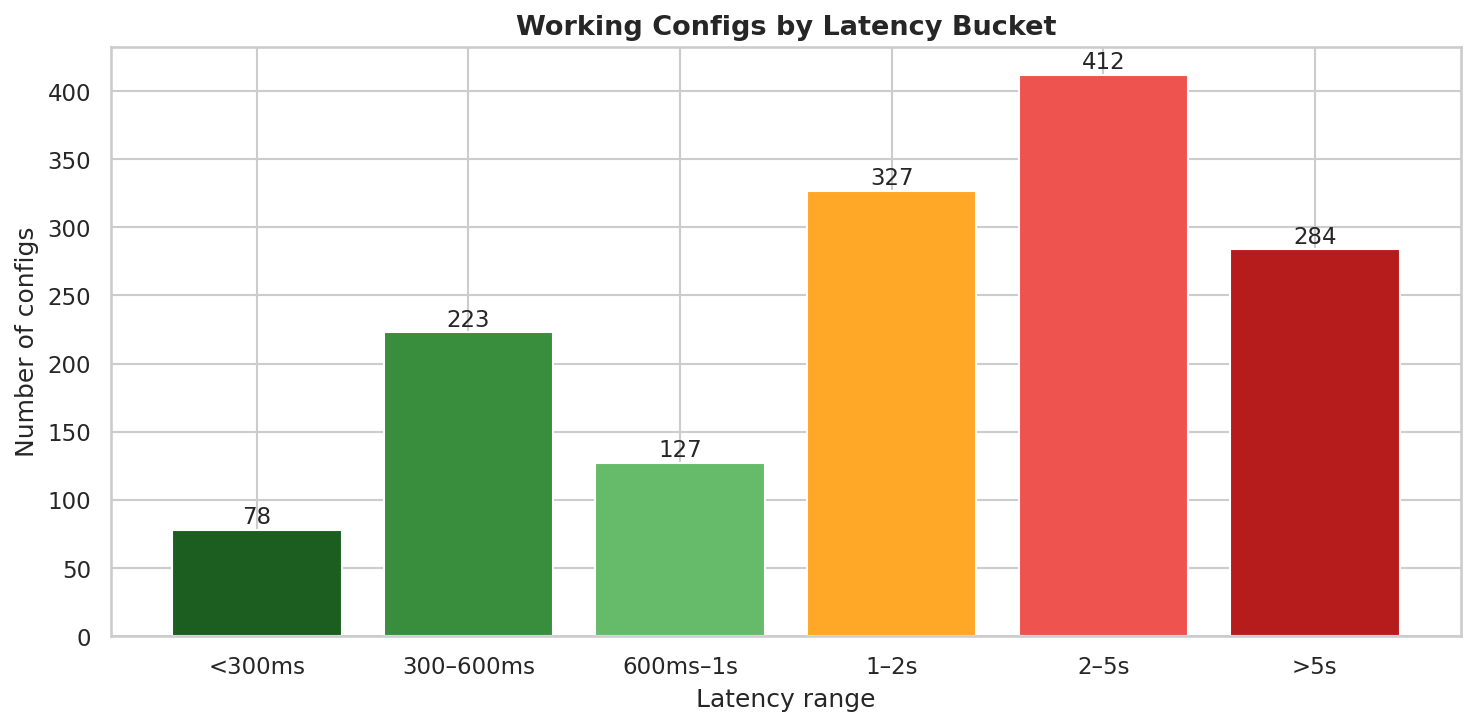
\includegraphics[width=0.9\columnwidth]{latency_distribution.png}
    \caption{Latency distribution across all reachable configurations (left, capped at 5000\,ms; median 1848\,ms, mean 3023\,ms) and latency by protocol as a box-plot (right). Hysteria2 shows the lowest median latency.}
    \label{fig:latency_distribution}
\end{figure}

Furthermore, studying this information from crash-free aspects demonstrates which proxy protocols have the most harmony with their configuration format.
The overall availability rate of 1.26\% across 115,042 configurations confirms that the free proxy ecosystem is characterized by severe configuration staleness, with the vast majority of published configurations pointing to offline or unreachable servers.

Another aspect of performance is latency distribution.
Due to different server locations of each configuration, they finish the proxy handshake within different durations.
The results show VLESS and VMess take significantly more time to process with respect to Hysteria2, with a mean latency of 3,023 ms and a median latency of 1,848 ms across all working configurations.

\subsection{Machine Learning Analysis}
The performance of machine learning models on the proxy configuration dataset reveals important structural properties of the subscription ecosystem~\cite{deep_packet2020}.
By applying Random Forest, Gradient Boosting, Logistic Regression, and a Multi-Layer Perceptron (MLP) to predict configuration availability from static metadata (protocol, port, and port class), the best achievable ROC-AUC score is approximately 0.76.
This demonstrates that static configuration metadata has limited but non-trivial predictive power for availability, and a significant portion of reachability depends on real-time server infrastructure conditions.

\begin{figure}[htbp]
    \centering
    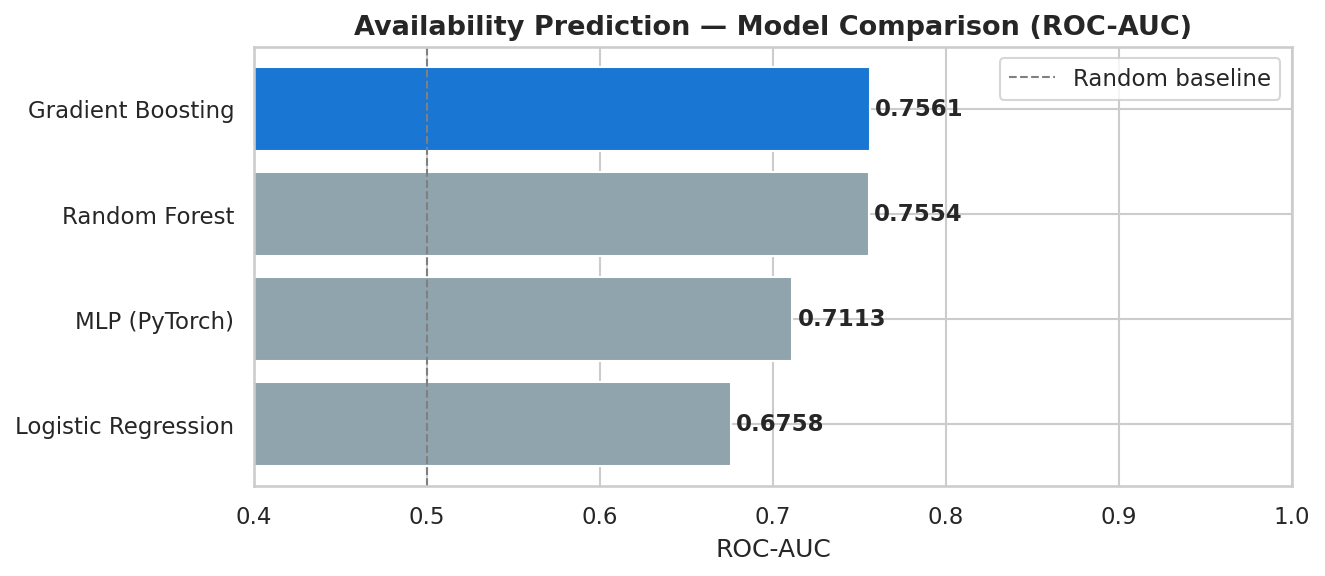
\includegraphics[width=0.9\columnwidth]{ml_model_comparison.png}
    \caption{Availability prediction model comparison by ROC-AUC. Gradient Boosting achieves the best score (0.756), followed by Random Forest (0.755), MLP (0.711), and Logistic Regression (0.676). All models outperform the random baseline (0.5).}
    \label{fig:ml_comparison}
\end{figure}

\begin{table}[t]
\centering
\caption{Ranking of Machine Learning Models by Availability Prediction (ROC-AUC).}
\label{tab:ml_model_ranking}
\renewcommand{\arraystretch}{1.2}
\resizebox{\linewidth}{!}{%
\begin{tabular}{c l c c}
\hline
\textbf{Rank} & \textbf{Model} & \textbf{ROC-AUC} & \textbf{F1-macro} \\
\hline
\textbf{1} & Gradient Boosting   & 0.756 & -- \\
\textbf{2} & Random Forest       & 0.755 & -- \\
\textbf{3} & MLP (PyTorch)       & 0.711 & -- \\
\textbf{4} & Logistic Regression & 0.676 & -- \\
\hline
\end{tabular}%
}
\end{table}

Furthermore, a crucial observation pertains to latency prediction.
The results of the study demonstrate that latency is not predictable from static configuration metadata alone (Gradient Boosting R$^2 < 0$), and they will vary after a while due to server load changes.
In fact, latency is driven by real-time network conditions (server load, routing path, and congestion) that are invisible in static configuration metadata.

\subsection{Discussion and Key Findings}
The results of this study demonstrate that proxy protocols have different behavior in providing reachable configurations.
The most robust protocol for this task is Hysteria2 with a significant gap with respect to other protocols.
On the other hand, for geographic distribution of reachable exit nodes, Germany is the most robust country to provide more reachable configurations with a large gap with respect to other countries.
Furthermore, this study shows that the analysis of the generated connectivity records is possible to do with several aspects to understand different dimensions of the generated proxy configurations.

\section{Conclusion and Future Work}
At the end of this project, there are several key findings.
Some of the most important findings are related to PAVE implementation.
The results of this project demonstrate that the implemented PAVE for proxy configurations is a practical and effective approach for testing connectivity and generating reachability records.
By considering many important aspects of the implementation, such as containerization, automation, and scalability, the PAVE is able to handle a wide range of configurations and test their connectivity in a reliable manner.

Another important finding is related to the robustness and performance of different proxy protocols.
The results of the study show that there are significant differences in the behavior of different protocols, both in terms of their ability to successfully provide reachable configurations and in terms of the geographic distribution of their exit nodes.

Furthermore, a crucial observation pertains to the proxy configuration and distribution.
The results of the study demonstrate that the published and freely available proxy configurations for protocols are not always reachable and accurate, and they will be unreachable after a while (Configuration Staleness).
In fact, proxy operators are adding new configurations and servers to their channels continuously without removing expired endpoints.

In conclusion, this project provides a comprehensive and practical solution for testing proxy connectivity and generating reachability records for free proxy configurations, and also provides a detailed analysis of the robustness and performance of different proxy protocols and their geographic infrastructure.

This project has focused on capturing proxy connectivity that uses the TCP~\cite{rfc793} and UDP~\cite{rfc768} protocols.
Despite the fact that TCP and UDP are the most widely used transports for proxy protocols, there are still many proxy services that use other transport mechanisms, such as WebSocket~\cite{rfc6455} over CDN or GRPC~\cite{grpc} over HTTP/2.
For future work, it would be interesting to extend the PAVE to support capturing proxy connectivity that uses non-standard transport layers.
Future work can explore lower layers of the network stack to capture proxy interactions, using tools such as pcap~\cite{libpcap} or tools based on eBPF~\cite{ebpf_io}.

In this project, the UI exploration component of the PAVE is based on a simple random testing strategy by the curl tool, which is a built-in tool in the Linux SDK.
For future work, it would be interesting to explore the use of AI-driven techniques for configuration exploration, such as reinforcement learning or evolutionary algorithms.
These techniques can potentially learn more effective exploration strategies over time, and can adapt to the specific characteristics of different proxy server implementations.

In this project, the PAVE is primarily focused on dynamic analysis of proxy connectivity.
At the end of the PAVE results, it is observable that there are some configurations that PAVE is not able to establish any proxy connectivity for, and it cannot cross their security barriers.
For future work, it would be interesting to explore the integration of the PAVE with static analysis tools to break the security barriers of configurations, and especially TLS certificate pinning bypass.
However, it is important to consider the ethical implications of such an approach, and to ensure that it is used in a responsible and legal manner.

\newpage

\bibliographystyle{IEEEtran}
\bibliography{references}

\end{document}